\documentclass[11pt,a4paper]{report}
%\fontfamily{cmss}
\hfuzz=9999pt % "fix" hbox overfull
%Path relative to the .tex file containing the \includegraphics command
\usepackage{graphicx}
\usepackage{hyperref}
\hypersetup{
    colorlinks=true,
    linkcolor=blue,
    filecolor=magenta,      
    urlcolor=blue
}

\begin{titlepage}
\title{BU551V - Applied Econometrics \\ Lecture Notes}
\author{Rodrigo Miguel}
\date{\today}
\end{titlepage}



\begin{document}
\maketitle
\tableofcontents

\chapter{Lecture 1}
\section{What is statistics?}
Statistics is the science of uncertainty.
\begin{itemize}
    \item What \textit{could} be;
    \item What \textit{might} be;
    \item What \textit{probably} is.
\end{itemize}
Statistics can be divided into two:
\begin{itemize}
    \item \textbf{Descriptive statistics:} Used to summarize information (how many), describe in a concise and easy to understand way.
    \item \textbf{Inferential statistics:} Asks about what we can learn from the population in the sample.
\end{itemize}
\subsection{Example}
If an airline is selling tickets to a flight with only 100 seats. A safe solution is to accept only 100 reservations. However, due to the human nature, cancellations and no-show-ups might happen. What would be the optimal number of reservations the airline should make?

\section{Statistical Inference}
\subsection{Statistical Inference}
Is used when we want to learn about a population given a sample/subset.
\subsection{Steps to Make a Statistical Inference}
\begin{itemize}
    \item Identify the population of interest;
    \item Specify a model for the population relationship of interest that contains unknown parameters.
    \item Obtain a \textbf{random} sample from the population.
    \item Estimate the parameters using the sample.
\end{itemize}
\subsection{Random Sample}
A \textbf{Random Sample} is a set of random variables (RVs) that follow a probability density function (pdf) $f(y,\theta)$.
\\When the RVs are from a random sample with $f(y,\theta)$ density, they are said to be \textbf{independent and identically distributed}.
\\Random samples can be assumed to be drawn from a normal distribution. Its population can be characterized by two parameters:
\begin{itemize}
    \item Mean $\mu$;
    \item Variance $\sigma^2$.
\end{itemize}
Usually we are only interested in $\mu$, however, in some cases, we also need to know $\sigma^2$.
\subsection{Estimators}
An estimator is a rule that assigns a value of $\theta$ to the sample.
\\For an actual realized sample, the estimate is just the average in the sample:
\[\overline{y} = \frac{(y_1 + y_2 + ... + y_n)}{n}\]

\subsection{General Expression for Estimators}
An estimator \textit{W} of a parameter $\theta$ can be expressed as an abstract formula:
\[W = h(Y_1, Y_2, ..., Y_n)\], where \textit{h} is an unknown function.
\\When we plug a set of actual observations ${y_1, y_2, ... y_n}$ into the function h, we obtain an estimate of $\theta$.

\section{Choosing an estimator}
To choose an estimator, criteria needs to be followed so that an estimator with "desirable" properties is correctly chosen. Here's the several properties that are used as choosing criteria:
\begin{itemize}
    \item Unbiasedness;
    \item Efficiency;
    \item Consistency.
\end{itemize}

\section{Unbiasedness}
An estimator of $\theta$ is \textbf{unbiased} if: \[E(W) = \theta\]
This does, however, \textbf{not} mean that an estimate in a particular sample is equal to $\theta$.
\\It means that:
\begin{enumerate}
    \item We draw random samples from the population many times;
    \item Compute an estimate each time;
    \item Average these estimates over all random samples;
    \item Then we obtain the true parameter $\theta$.
\end{enumerate}

\subsection{Bias of an estimator}
An estimator of $\theta$, W, is a biased estimator if:
\[E(W) \neq \theta\]
Its bias is defined as:
\[Bias(W) \equiv E(W) - \theta\]

\begin{figure}[h]
    \centering
    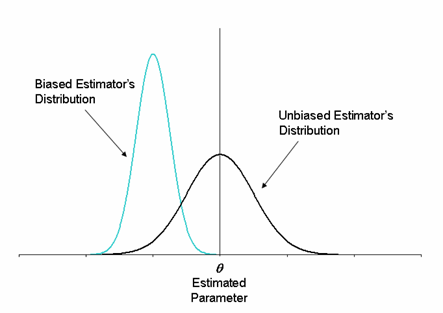
\includegraphics[width=\textwidth]{images/unbiasedness.png}
    \caption{An unbiased estimator W, and an estimator with positive bias, $W_2$.}
    \label{Unbiasedness}
\end{figure}

\begin{itemize}
    \item An estimator being unbiased does not necessarily mean it's a good estimator.
\end{itemize}

\section{Efficiency}
\subsection{Sampling Variance of Estimators}
\begin{itemize}
    \item Unbiasedness ensures that the distribution of an estimator has a mean value which is equal to the true parameter $\theta$.
    \item It is a good property but not enough.
    \item We want an estimator that can show us a mean value equal to $\theta$ and centred around $\theta$ as tightly as possible.
\end{itemize}
To measure how spread out a distribution is, we use the variance, Var(W). To calculate it, we use the sample average as an estimator $w = \overline{Y}$.
\paragraph{Summary}
If ${Y_1, ..., Y_n}$ is a random sample from a population with mean $\mu$ and variance $\sigma^2$:
\begin{itemize}
    \item $\overline{Y}$ has a mean $\mu$ and variance $\frac{\sigma^2}{n}$
\end{itemize}
\subsection{Which estimator is better?}
Among unbiased estimators, we prefer the estimator with the smallest variance.

\section{Consistency}
Consistency, is a property that captures how estimators improve as the sample size, \textit{n}, increases.
\subsection{Example}
\begin{itemize}
    \item An estimator $\overline{Y}$ has $Var(\overline{Y}) = \frac{\sigma^2}{n}$, meaning that as \textit{n} gets larger, the estimator improves.
    \item An estimator $Y_1$ has $Var(Y_1) = \sigma^2$, meaning no improvement even if \textit{n} gets larger.
\end{itemize}
\subsection{Importance of Consistency}
Consistency is a minimum requirement of an estimator used in econometrics.
\subsection{Law of Large Number}


\end{document}